\documentclass[a4paper, 11pt]{article}

\usepackage[utf8]{inputenc}
\usepackage[english]{babel}

\usepackage{hyperref}

\usepackage{standalone}

\usepackage{lscape}

\usepackage{graphicx}
\usepackage{subfig}
\usepackage{tikz}

\usepackage{floatrow}
\captionsetup{labelsep=period}

\usepackage{listings}

\usepackage{fullpage}

\begin{document}
	\begin{centering}
		\Large{\textbf{Progress Report}}\\
		\large{\today}
~\\
		Oussama ENNAFII\\
		Directors: Cl\'ement Mallet \& Florent Lafarge \\
		Advisor: Arnaud Le Bris \\

	\end{centering}


	\section{The Dataset:}
~\\

	We have decided earlier in June to work on Nantes and Dijon in addition to
	Elancourt. As I explained later, the $3DS$ data for these regions are not
	well formated so that I can retrieve the building entities. In order to
	establish first a whole pipeline. I will deal with those regions later using
	the $CityGML$ data. In consequence, I will continue to work on Elancourt
	only, for now.\\

	I have also relabelled the zone I had labelled before. That is due to the fact
	that the taxonomy has evolved during the annotation. I have used $QGIS$ to
	annotate buildings' projected facets based on errors they showed.\\

	The errors have been subdivided, based on the labelling, into three classes:

	\begin{itemize}
		\item[-] Unqualified Building Errors: Concerns the buildings that will not
		be taken into consideration,
		\item[-] Building Errors: encompasses the errors that affect the whole
		building (corrensponds roughly to $LoD0$ and $LoD1$ errors),
		\item[-] Facet Errors: concerns errors affecting only a facet.
	\end{itemize}

	Here are some statistics over the labelled Dataset comprizing $502$ buildings:

	\begin{itemize}
		\item ratio of \textbf{Building} errors among all errors: $0.2408$
		\begin{itemize}
			\item[-] ratio of \textbf{Over Segmentation} errors:
			\begin{itemize}
				\item[(i).] among \textbf{Building} errors:  $0.1365$
				\item[(ii).] among all files:  $0.03287$
			\end{itemize}
			\item[-] ratio of \textbf{Under Segmentation} errors:
			\begin{itemize}
				\item[(i).] among \textbf{Building} errors:  $0.4177$
				\item[(ii).] among all files:   $0.1006$
			\end{itemize}
			\item[-] ratio of \textbf{Footprint} errors:
			\begin{itemize}
				\item[(i).] among \textbf{Building} errors:  $0.4839$
				\item[(ii).] among all files:  $0.1165$
			\end{itemize}
			\item[-] ratio of \textbf{Altimetric} errors:
			\begin{itemize}
				\item[(i).] among \textbf{Building} errors:  $0.0165$
				\item[(ii).] among all files:  $0.0040$
			\end{itemize}
		\end{itemize}
		\item ratio of \textbf{Facet} errors among all errors: $0.81657$
		\begin{itemize}
			\item[-] ratio of \textbf{Over Segmentation} errors:
			\begin{itemize}
				\item[(i).] among \textbf{Facet} errors:  $0.8830$
				\item[(ii).] among all files:  $0.7203$
			\end{itemize}
			\item[-] ratio of \textbf{Under Segmentation} errors:
			\begin{itemize}
				\item[(i).] among \textbf{Facet} errors:  $0.0842$
				\item[(ii).] among all files:   $0.0687$
			\end{itemize}
			\item[-] ratio of \textbf{Mis Segmentation} errors:
			\begin{itemize}
				\item[(i).] among \textbf{Facet} errors:  $0.0806$
				\item[(ii).] among all files:  $0.0657$
			\end{itemize}
			\item[-] ratio of \textbf{Slope} errors:
			\begin{itemize}
				\item[(i).] among \textbf{Facet} errors:  $0.0327$
				\item[(ii).] among all files:  $0.0267$
			\end{itemize}
		\end{itemize}
		\item ratio of \textbf{Unqualified} errors among all errors: $0.0876$
		\begin{itemize}
			\item[-] ratio of \textbf{Half Building} errors:
			\begin{itemize}
				\item[(i).] among \textbf{Unqualified} errors:  $0.8636$
				\item[(ii).] among all files:  $0.0757$
			\end{itemize}
			\item[-] ratio of \textbf{Change Building} errors:
			\begin{itemize}
				\item[(i).] among \textbf{Unqualified} errors:  $0.0455$
				\item[(ii).] among all files:   $0.0040$
			\end{itemize}
			\item[-] ratio of \textbf{Occlusion} errors:
			\begin{itemize}
				\item[(i).] among \textbf{Unqualified} errors:  $0.0455$
				\item[(ii).] among all files:  $0.0040$
			\end{itemize}
			\item[-] ratio of \textbf{Unknown} errors:
			\begin{itemize}
				\item[(i).] among \textbf{Unqualified} errors:   $0.0455$
				\item[(ii).] among all files:  $0.0040$
			\end{itemize}
		\end{itemize}
	\end{itemize}


	\begin{landscape}
		\begin{figure}
			\begin{center}
				\includestandalone[mode=buildnew, scale=.78]{mind_map}
				\caption{\label{fig::mindmap_errors} Mind map representing the errors encountered during the annotation.}
			\end{center}
		\end{figure}
	\end{landscape}

	\thisfloatsetup{heightadjust=object}
	\begin{figure}
		\begin{center}
			\ffigbox
			{
				\ffigbox[\FBwidth]
				{
					\begin{subfloatrow}[4]
						\captionsetup{labelformat=brace, justification=raggedright}
						\ffigbox[\FBwidth]{\caption{Half Building.}\label{fig::half_building}}{\fbox{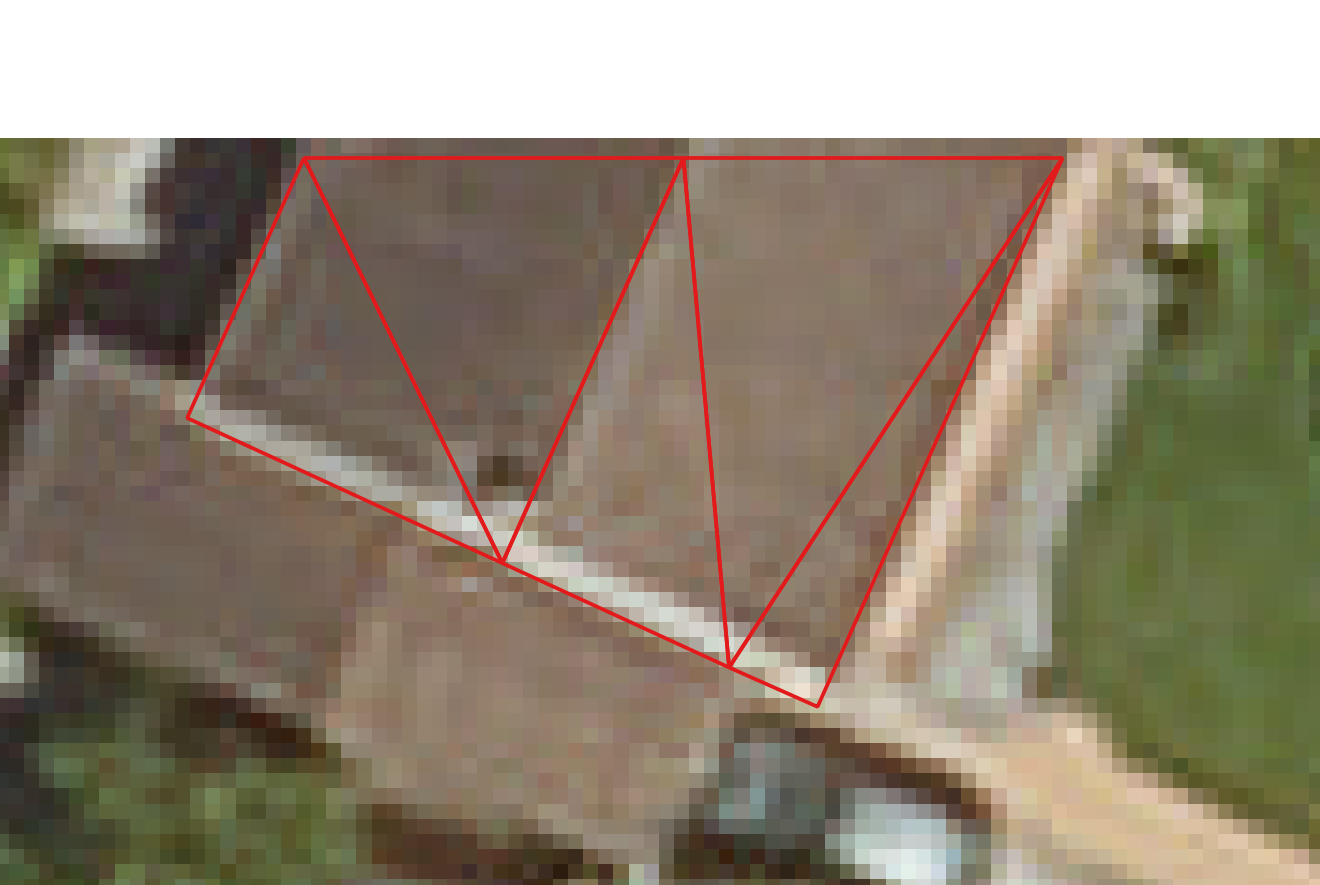
\includegraphics[width=.24\textwidth]{../images/raster/Unqualified_Errors/half_building}}}
						\ffigbox[\FBwidth]{\caption{Changed Building.}\label{fig::changed}}{\fbox{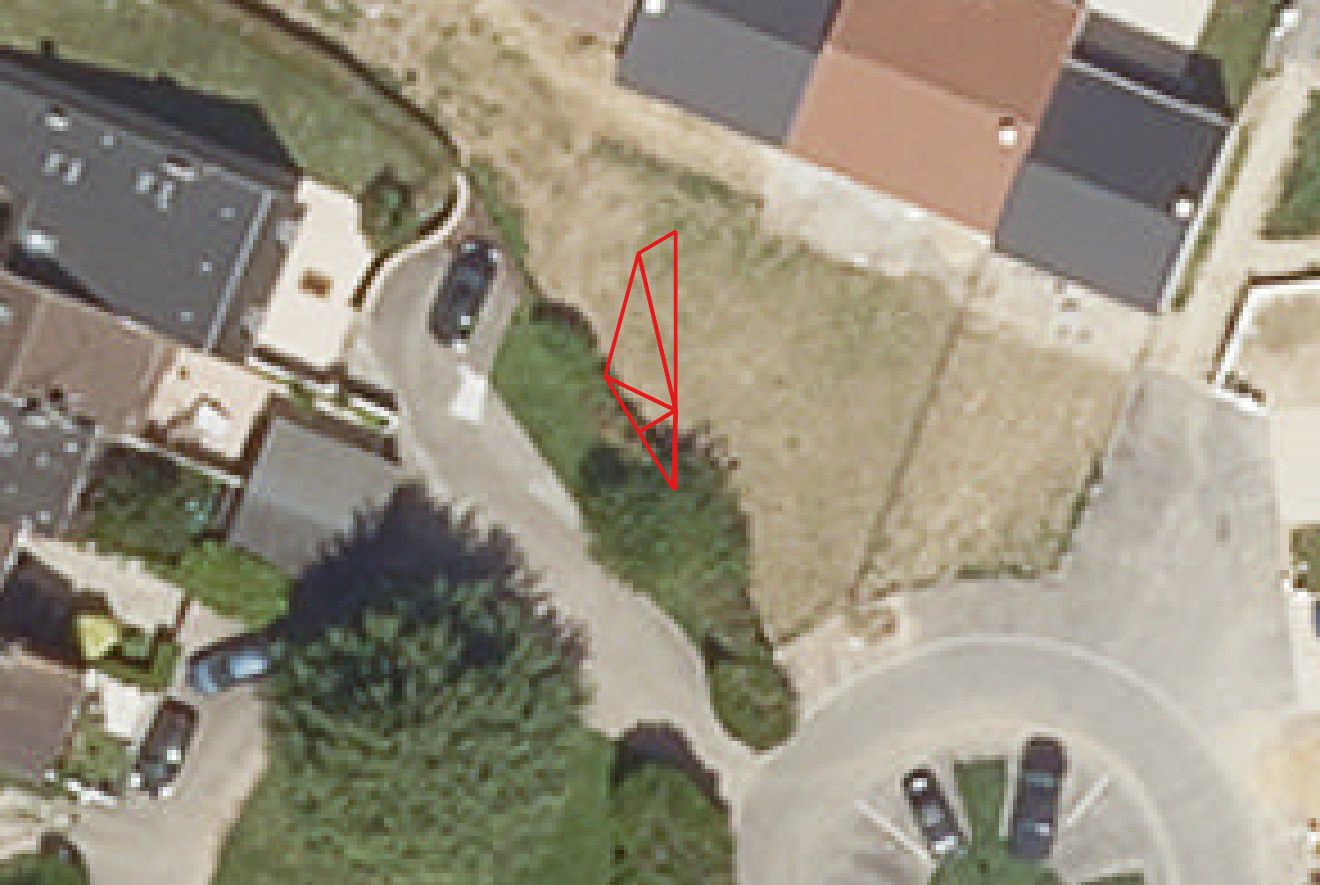
\includegraphics[width=.24\textwidth]{../images/raster/Unqualified_Errors/changed}}}
						\ffigbox[\FBwidth]{\caption{Occlusion.}\label{fig::occlusion}}{\fbox{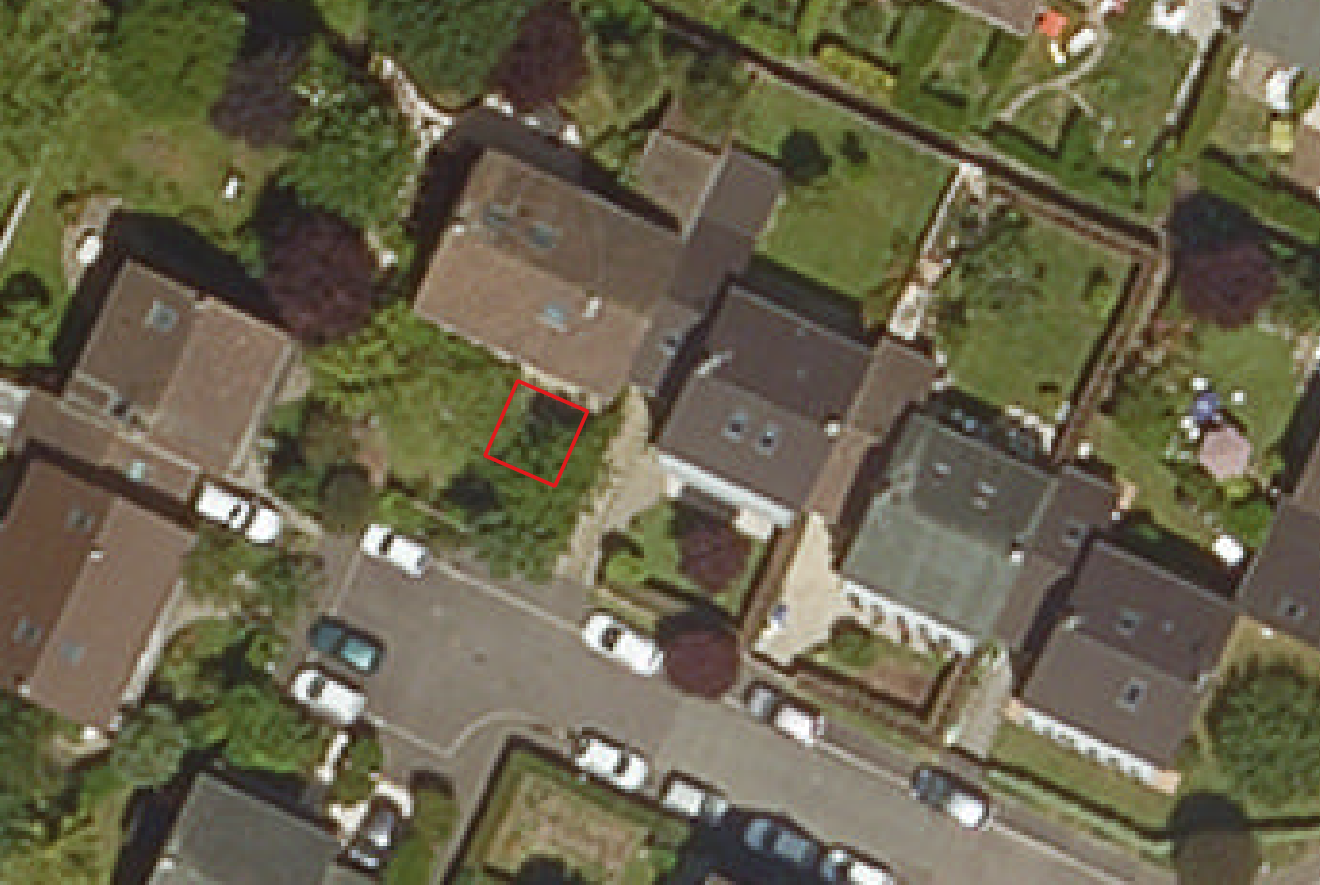
\includegraphics[width=.24\textwidth]{../images/raster/Unqualified_Errors/occlusion}}}
						\ffigbox[\FBwidth]{\caption{Unknown.}\label{fig::unknown}}{\fbox{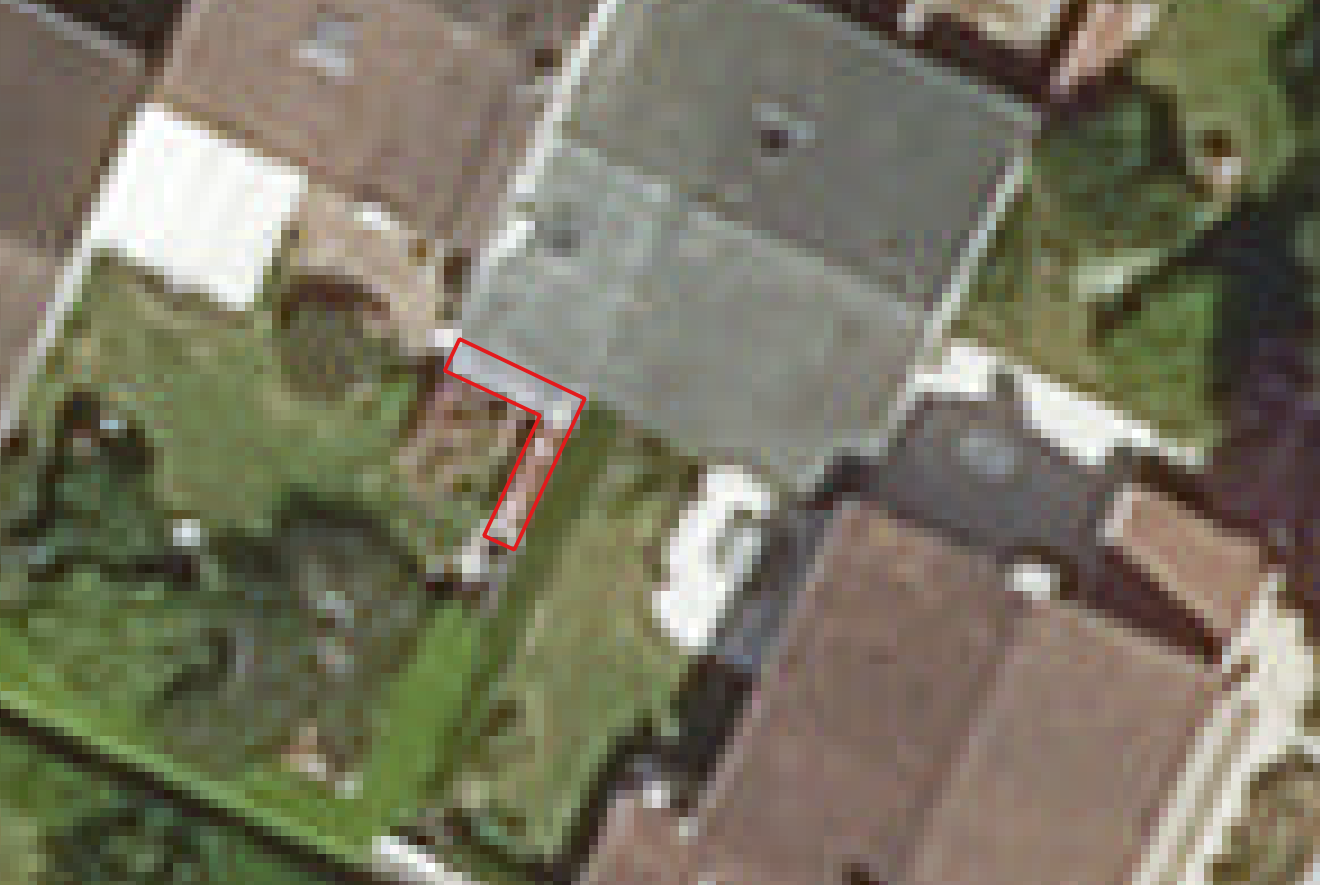
\includegraphics[width=.24\textwidth]{../images/raster/Unqualified_Errors/unknown}}}
					\end{subfloatrow}
				}
				{
					\caption*{\label{fig::unq_samples} (i). Samples of Unqualified building errors.}
				}
				\ffigbox[\FBwidth]
				{
					\begin{subfloatrow}[4]
						\captionsetup{labelformat=brace, justification=raggedright}
						\ffigbox[\FBwidth]{\caption{Under Segmentation.}\label{fig::under_bul}}{\fbox{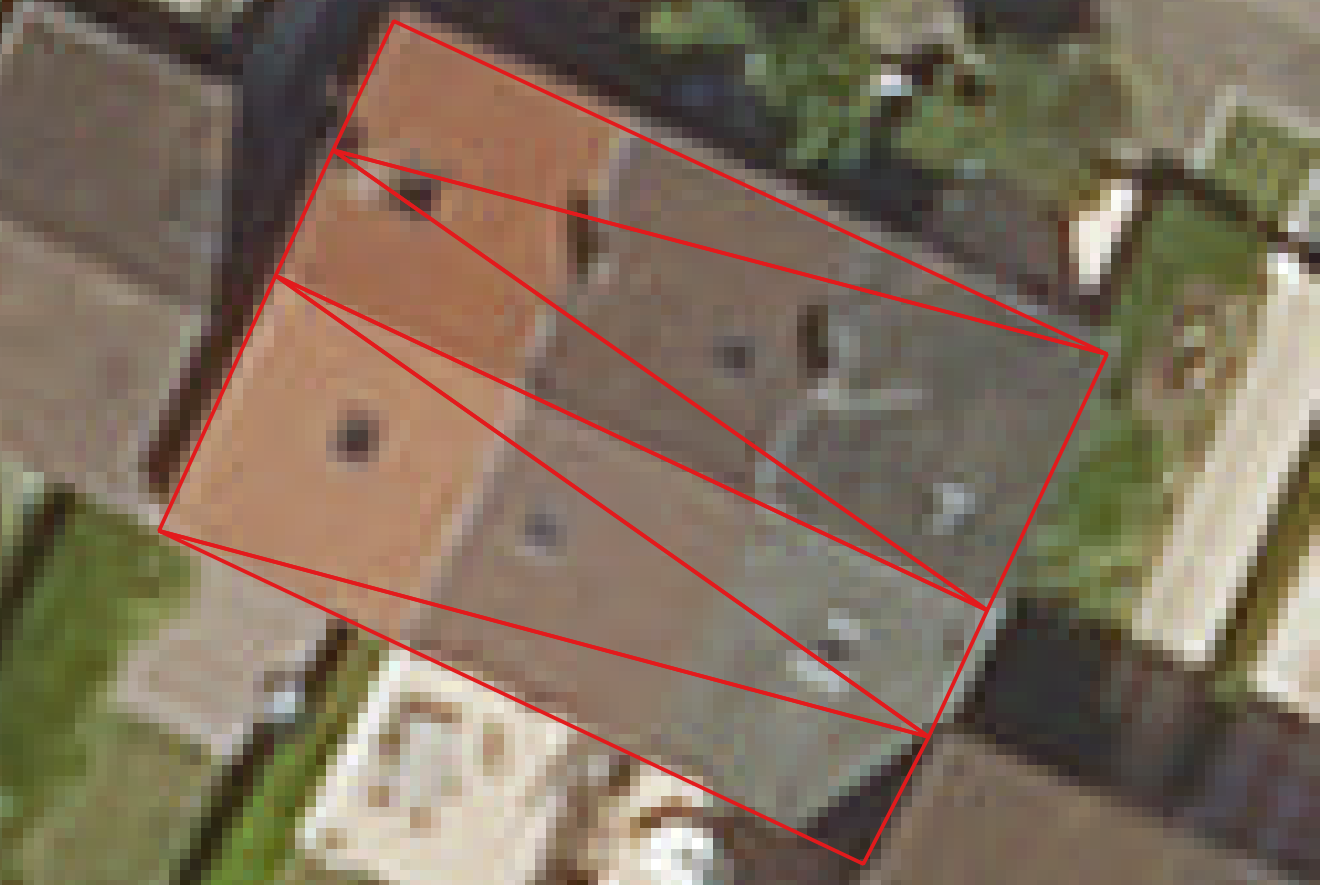
\includegraphics[width=.24\textwidth]{../images/raster/Building_Errors/under_segmentation}}}
						\ffigbox[\FBwidth]{\caption{Over segmentation.}\label{fig::over_bul}}{\fbox{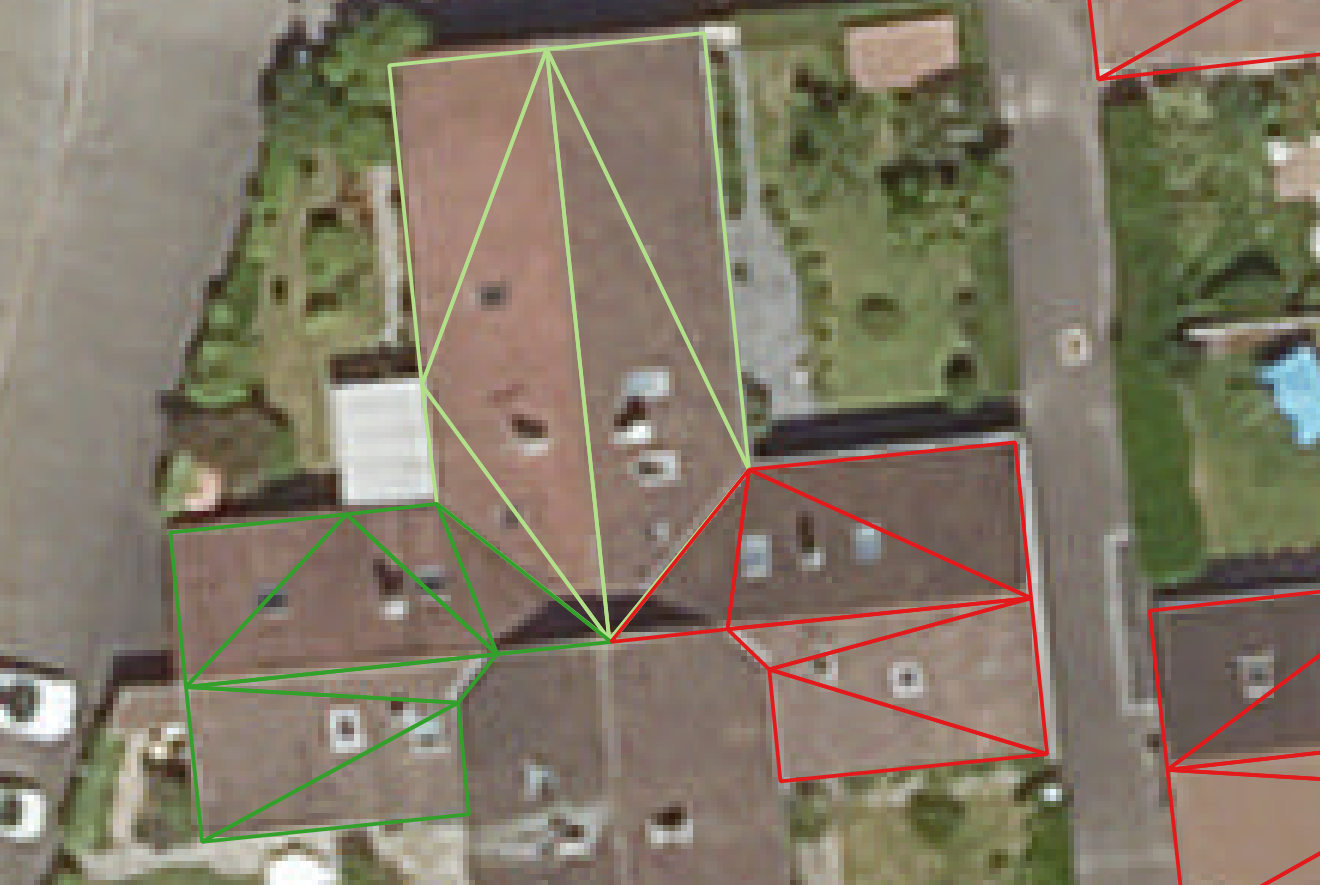
\includegraphics[width=.24\textwidth]{../images/raster/Building_Errors/over_segmentation}}}
						\ffigbox[\FBwidth]{\caption{Footprint.}\label{fig::footprint}}{\fbox{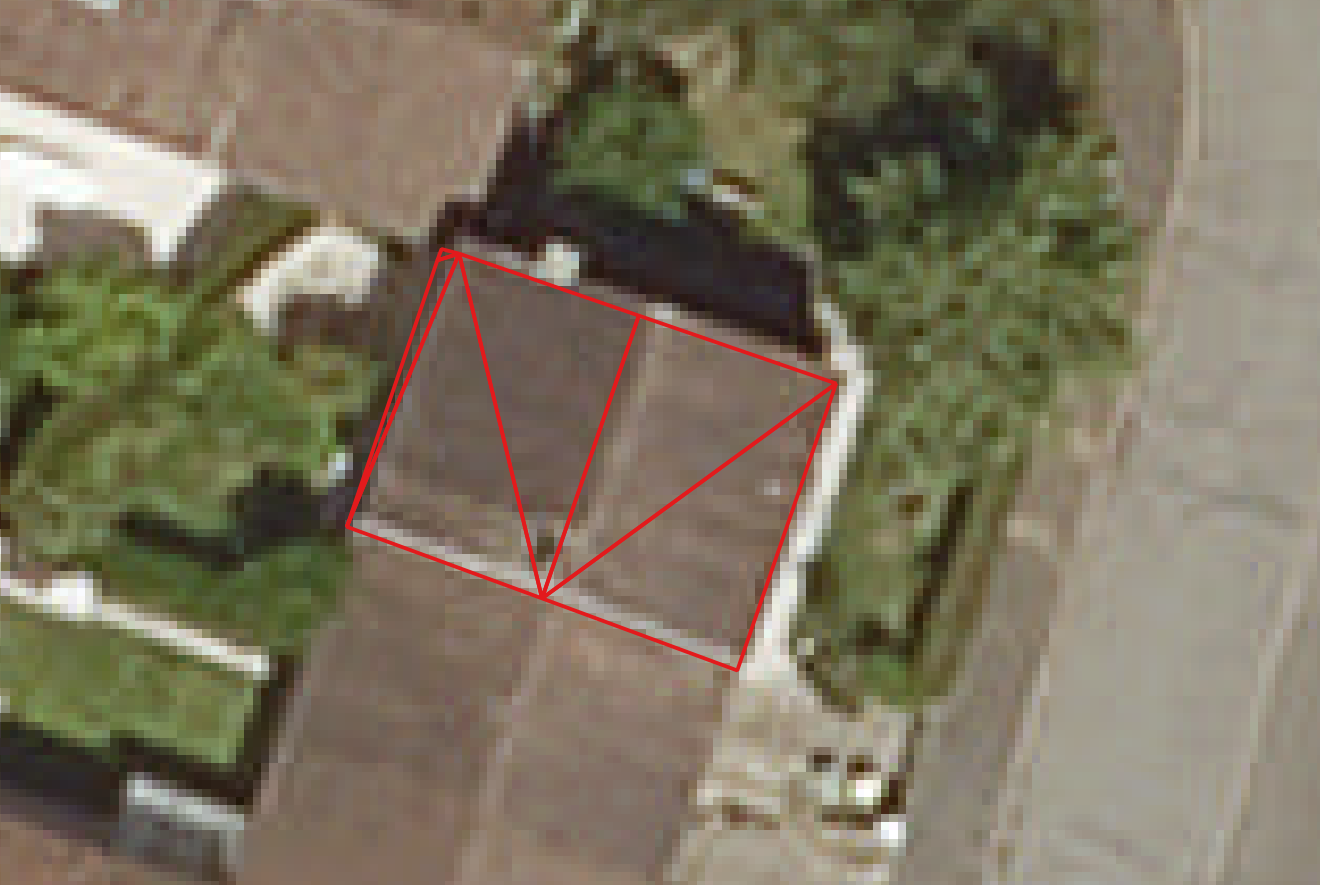
\includegraphics[width=.24\textwidth]{../images/raster/Building_Errors/footprint}}}
						\ffigbox[\FBwidth]{\caption{Altitude.}\label{fig::too_low}}{\fbox{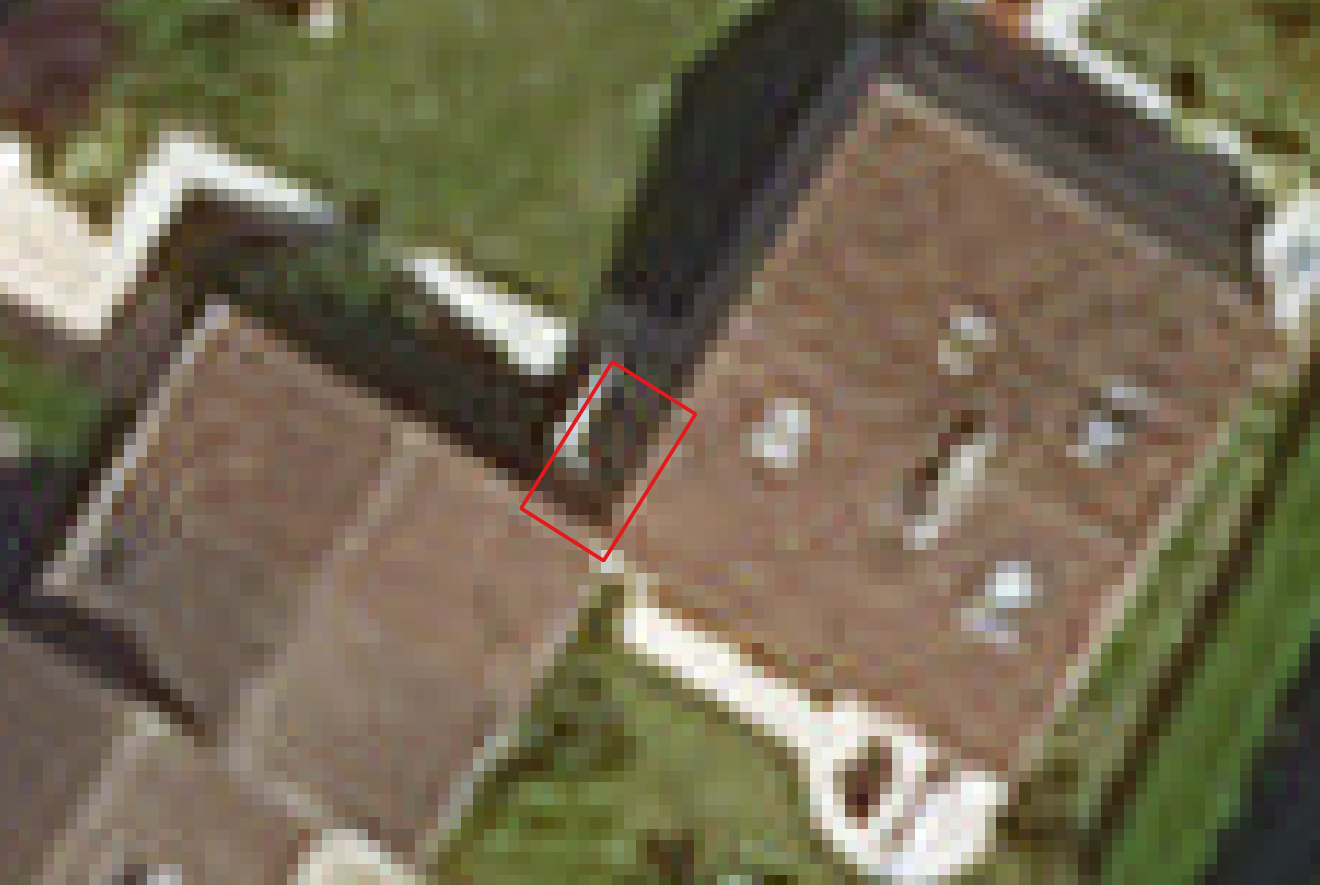
\includegraphics[width=.24\textwidth]{../images/raster/Building_Errors/altimetric}}}
					\end{subfloatrow}
				}
				{
					\caption*{\label{fig::bul_samples} (ii). Samples of Building errors.}
				}
				\ffigbox[\FBwidth]
				{
					\begin{subfloatrow}[4]
						\captionsetup{labelformat=brace, justification=raggedright}
						\ffigbox[\FBwidth]{\caption{Under Segmentation.}\label{fig::under_fac}}{\fbox{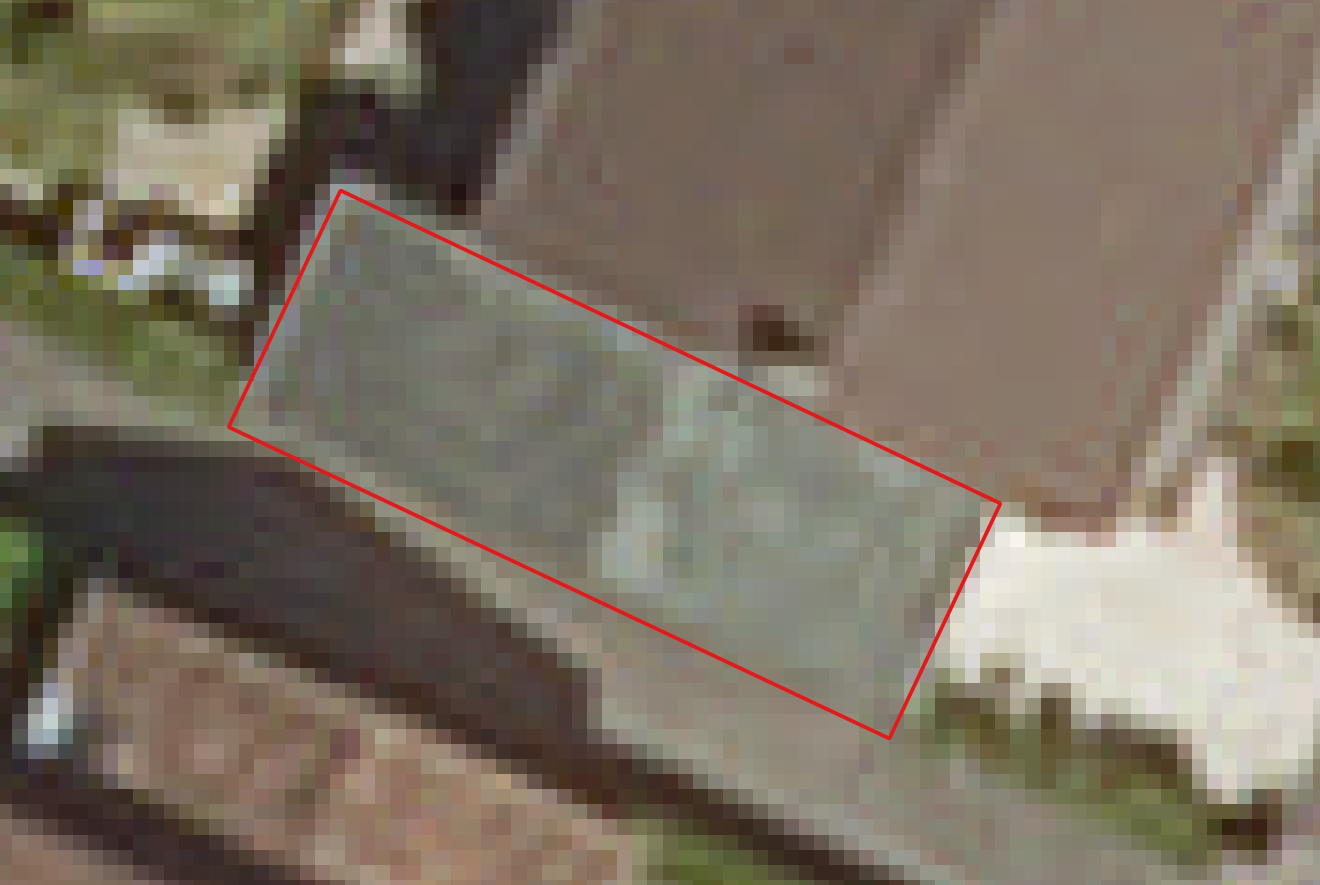
\includegraphics[width=.24\textwidth]{../images/raster/Facet_Errors/under_segmentation}}}
						\ffigbox[\FBwidth]{\caption{Over segmentation.}\label{fig::over_fac}}{\fbox{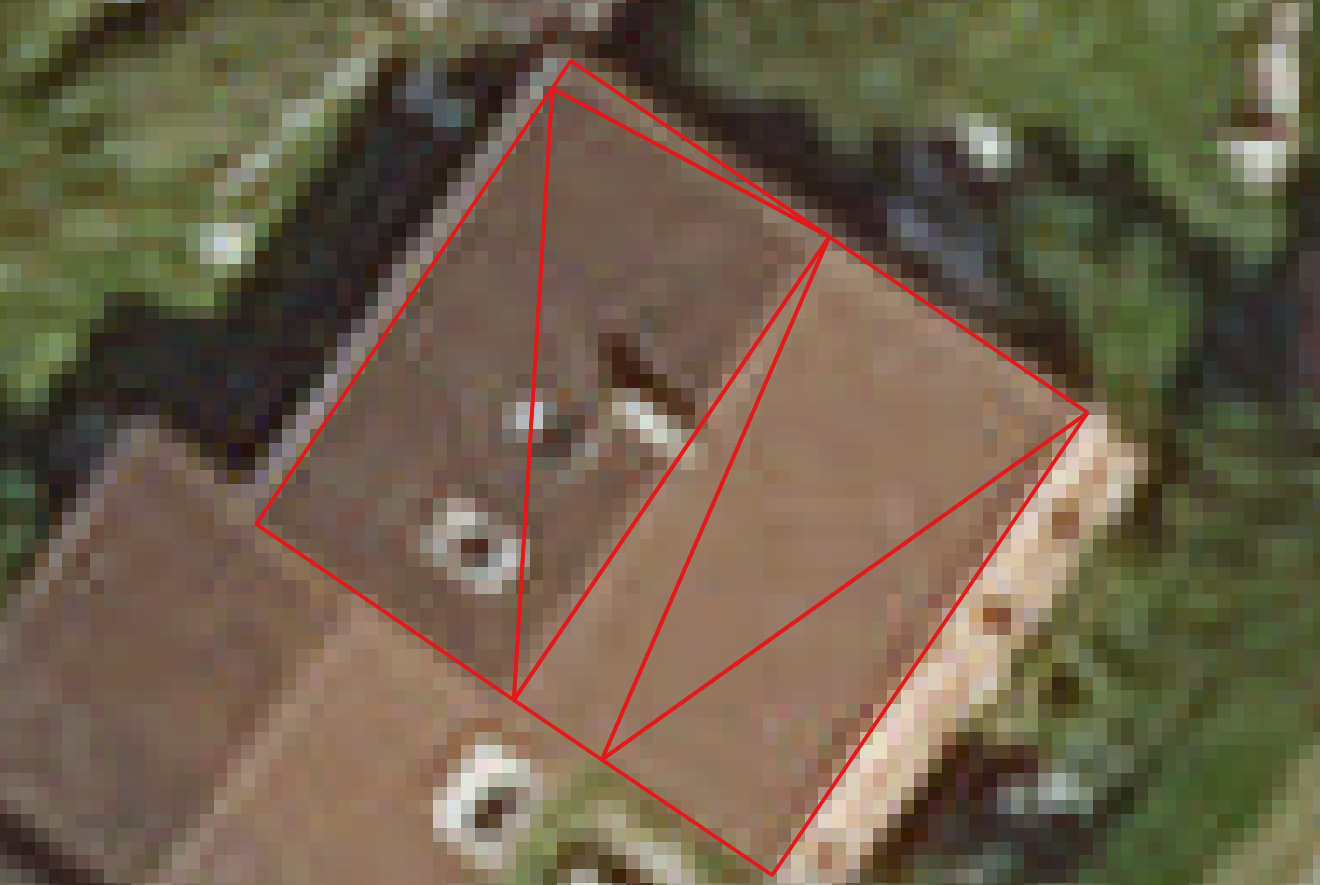
\includegraphics[width=.24\textwidth]{../images/raster/Facet_Errors/over_segmentation}}}
						\ffigbox[\FBwidth]{\caption{Mis Segmentation.}\label{fig::mis}}{\fbox{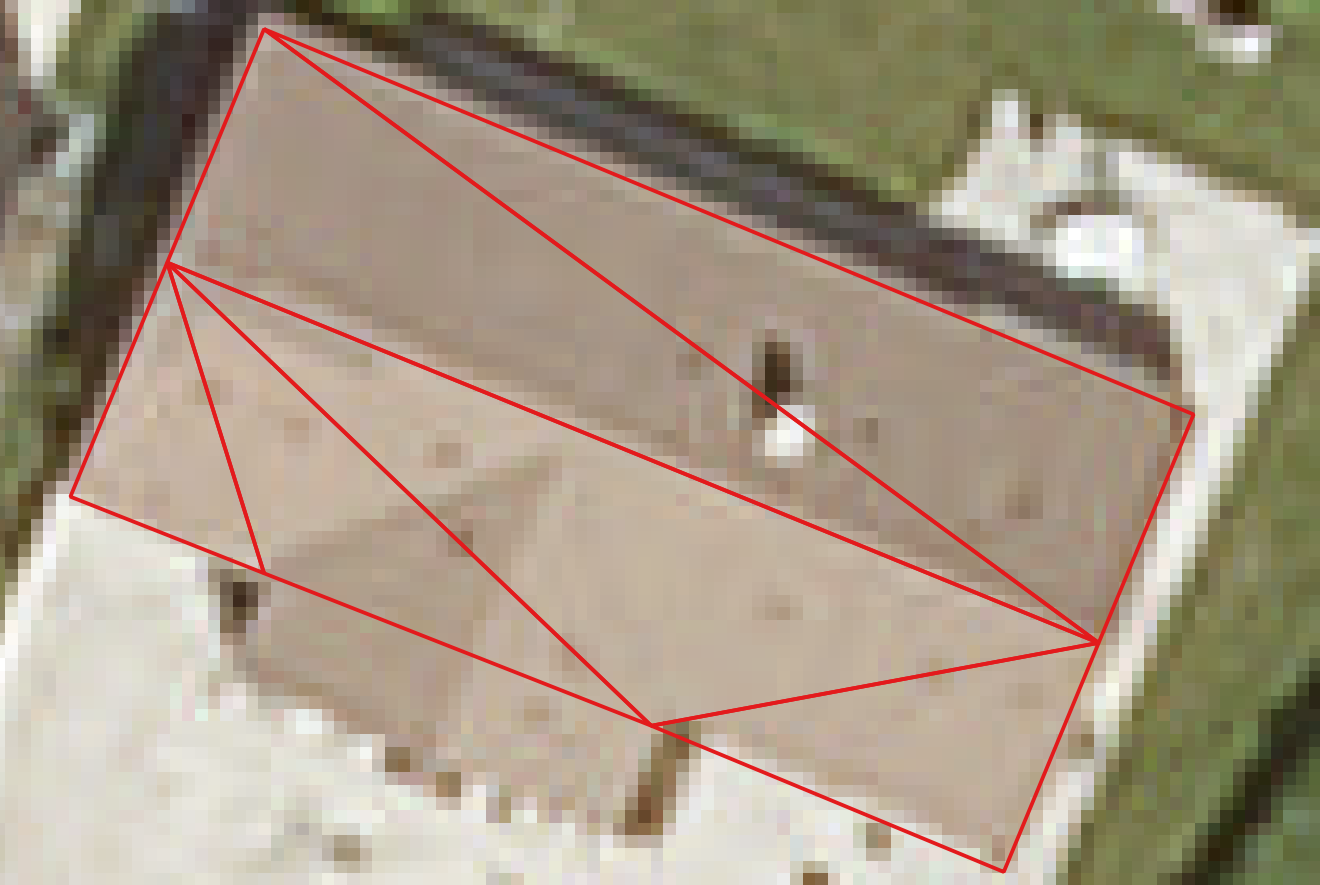
\includegraphics[width=.24\textwidth]{../images/raster/Facet_Errors/mis_segmentation}}}
						\ffigbox[\FBwidth]{\caption{Slope.}\label{fig::slope}}{\fbox{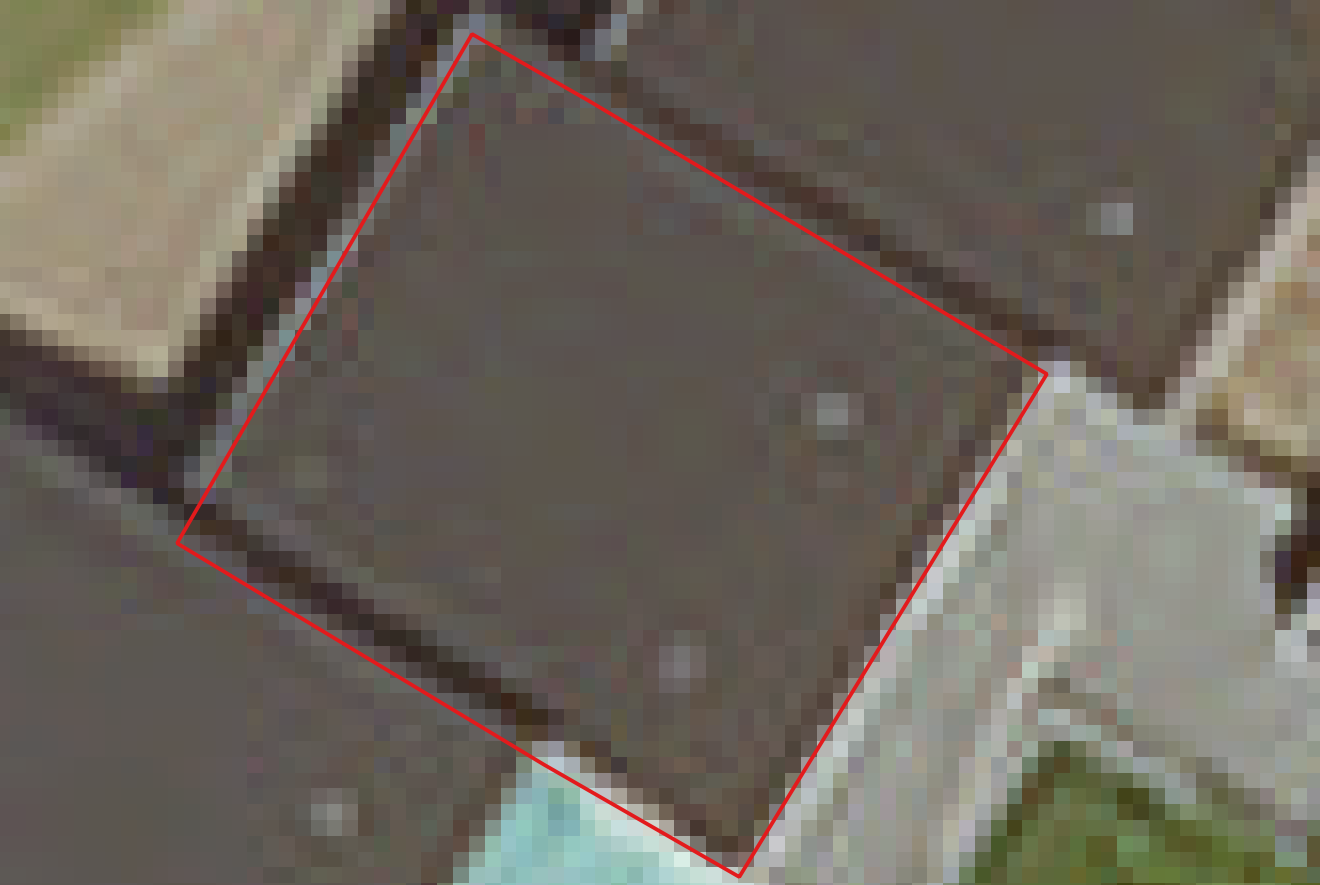
\includegraphics[width=.24\textwidth]{../images/raster/Facet_Errors/slope}}}
					\end{subfloatrow}
				}
				{
					\caption*{\label{fig::fac_samples} (iii). Samples of Facet errors.}
				}
			}
			{
				\caption{\label{fig::samples}Illustration of errors per class.}
			}
		\end{center}
	\end{figure}
	\clearpage

\section*{Attachments:}

\begin{itemize}
	\item[-] You can checkout the preprocessing code on
	\href{https://github.com/ethiy/proj.city}{Github}.
	\item[-] You can also check the feature extraction and classification code
	\href{https://github.com/ethiy/qualcity}{here}.
\end{itemize}

\end{document}
